\documentclass{beamer}
\usetheme{metropolis}           % Use metropolis theme
\usepackage[utf8]{inputenc}
\usepackage[danish]{babel}
\usepackage{../opstilling}
\usepackage{pgfplots}
\usepackage{tikz}
\usetikzlibrary{calc,patterns,decorations.pathmorphing,decorations.markings}
\title{SRP: Den dæmpede harmoniske svingning}
\date{\today}
\author{Mikkel B. Goldschmidt}
\institute{TalentCampDK}
\begin{document}
  \maketitle
  \section{Studieretningsprojektet (SRP)}
  \begin{frame}{Hvad er en SRP?}
  \textbf{Studieretningsprojektet}
	\begin{itemize}
		\item De flestes gymnasieelevers største frygt
		\item Opgave i 2 fag (minimum 1 linjefag på A-niveau)
		\item 2 ugers skrive tid (1 uge på HTX)
		\item Tæller for det samme som et A-fag
	\end{itemize}
  \end{frame}
  
  \begin{frame}{Mikkels SRP}
  	\textbf{Fag}: Matematik + Fysik\\
  	\textbf{Overemne}: Mekanik og \alert{differentialligninger}\\
  	\textbf{Fokus}: Dæmpede harmoniske svingninger og den andenordens homogene lineære differentialligning\\
  	\textbf{Problemformulering}:  .....
	  
  
  \end{frame}
  \begin{frame}{Problemformulering}
  \emph{Opskriv ved hjælp af Newtons 2. lov differentialligninger, der beskriver harmoniske og
dæmpede svingninger. Beskriv herunder dæmpningsleddet.

Gør matematisk rede for løsningsmetoder til lineære andenordens differentialligninger.

Kom ind på ikke lineære andenordens differentialligninger.
Udfør eksperimenter med harmoniske og dæmpede svingninger og analyser, hvordan
resultaterne kan beskrives matematisk. Diskuter herunder grundigt dæmpningsleddets
betydning for overensstemmelsen mellem teori og eksperiment.

Perspektiver til anvendelsen af mekaniske svingninger i teknologiske sammenhænge.}
  
  \end{frame}
  
\section{Problemet}

\begin{frame}{Opstil en model}

\textbf{For...}
\only<2->{\textbf{et lod i en fjedder!!!}}

\begin{center}
\only<3->{\opstilling{-1}}
\only<4->{\hspace{1cm}\opstilling{-0.5}}
\only<5->{\hspace{1cm}\opstilling{0}}
\only<6->{\hspace{1cm}\opstilling{-0.5}}
\end{center}

\end{frame}


\begin{frame}{Lidt om fjedre}



\only<1>{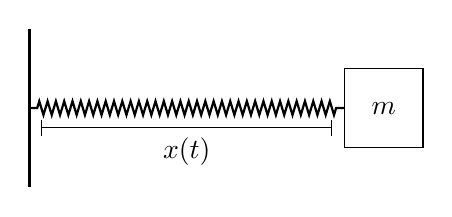
\begin{tikzpicture}
\pgfmathsetmacro{\xPos}{4}

\tikzstyle{spring}=[thick,decorate,decoration={zigzag,pre length=0.1cm,post length=0.1cm,segment length=3}]
\draw[very thick] (0,1) -- (0,-1);
\draw[spring](0,0) -- (\xPos,0) ;
\draw[|-|] (0.15,-0.25) -- (\xPos -0.15, -0.25) node[pos=0.5, below]{$x(t)$};
\draw (\xPos,-0.5) rectangle (\xPos + 1,0.5);
\node at (\xPos + 0.5,0) {$m$};
\end{tikzpicture}}
\only<2->{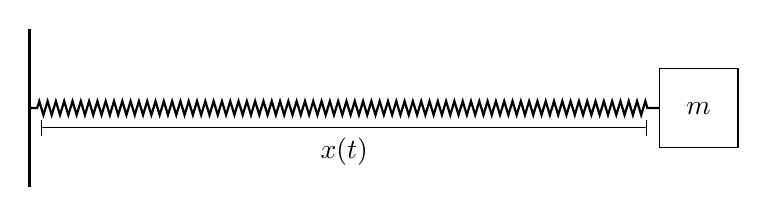
\begin{tikzpicture}
\pgfmathsetmacro{\xPos}{8}

\tikzstyle{spring}=[thick,decorate,decoration={zigzag,pre length=0.1cm,post length=0.1cm,segment length=3}]
\draw[very thick] (0,1) -- (0,-1);
\draw[spring](0,0) -- (\xPos,0) ;
\draw[|-|] (0.15,-0.25) -- (\xPos -0.15, -0.25) node[pos=0.5, below]{$x(t)$};
\draw (\xPos,-0.5) rectangle (\xPos + 1,0.5);
\node at (\xPos + 0.5,0) {$m$};
\end{tikzpicture}}

\vspace{0.5cm}

\metroset{block=fill}
\begin{block}{Hookes lov}
Accelerationen stiger proportionalt med udstrækningen af fjederen:
$$x''(t) = -\dfrac{k}{m} \cdot x(t)$$

$k$: fjederkonstanten\\
$m$: loddets masse
\end{block}

\end{frame}

\begin{frame}{Lidt om tyngdekraften}

\begin{center}
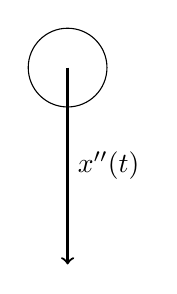
\begin{tikzpicture}
\draw (0,0) circle (0.5);
\draw[->, thick] (0,0) -- (0,-2.5) node[pos=0.5, right]{$x''(t)$};
\end{tikzpicture}
\hspace{2cm}
\only<2->{
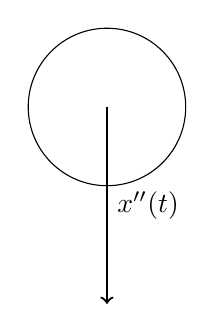
\begin{tikzpicture}
\draw (0,0) circle (1);
\draw[->, thick] (0,0) -- (0,-2.5) node[pos=0.5, right]{$x''(t)$};
\end{tikzpicture}}
\end{center}

\metroset{block=fill}
\begin{block}{Tyngdeloven}
Der er en konstant acceleration nedad på alle objekter - uanset masse.
$$x''(t) = -g$$

$g$: gravitationskonstanten\\
\vspace{0.2cm}

\end{block}

\end{frame}

\begin{frame}{Variable}
\begin{itemize}
	\item $t$: tiden efter der er givet slip
	\item $x(t)$: højden efter bevægelsens start
	\item $g$: tyngdeaccelerationen
	\item $m$: loddet vægt (masse)
	\item $k$: fjederens fjederkonstant
\end{itemize}

\end{frame}
\section{Forskellige modeller}
\begin{frame}{En simpel model}
Vi opsætter en model hvor der tages højde for fjeder og tyngdekraft:
$$x''(t) = \underbrace{-\dfrac{k}{m} \cdot x(t)}_{fjeder} \only<1-2>{\underbrace{-g\cdot m}_{tyngdekraft}}\pause \Leftrightarrow x''+\dfrac{k}{m}\cdot x \only<2>{+ g\cdot m}=0$$
\pause
\pause
Karakterligning: $r^2 + \frac{k}{m}\pause\Rightarrow r = \pm i \sqrt{\frac{k}{m}}$
\pause

Vi får altså (med en smule magi)
$$x(t)=C \cdot e^{i \sqrt{\frac{k}{m}}\cdot t}+D \cdot e^{-i \sqrt{\frac{k}{m}}\cdot t}\pause = A\cdot \sin (bt+\phi)$$

\end{frame}

\begin{frame}{Plot af model}
\begin{center}
\begin{tikzpicture}
\begin{axis}[
	title = Simpel model,
	xlabel = {$Tid/s$},
	ylabel = {$x(t)/cm$},
	xmin = 0,
	xmax = 8,
	ymin = -7,
	ymax = 7,
	minor y tick num=1,
	legend entries = {model, data},
]
\addplot[blue] table {pythonScripts/model1.plot};
\only<2->{
\addplot[red] table {pythonScripts/data.plot};}
\end{axis}
\end{tikzpicture}
\end{center}
\end{frame}

\begin{frame}{Plot af model}


\begin{center}
\begin{tikzpicture}
\begin{axis}[
	title = Simpel model,
	xlabel = {$Tid/s$},
	ylabel = {$x(t)/cm$},
	xmin = 0,
	xmax = 30,
	ymin = -7,
	ymax = 7,
	minor y tick num=1,
	legend entries = {model, data},
]
\addplot[blue] table {pythonScripts/model1.plot};
\addplot[red] table {pythonScripts/data.plot};
\end{axis}
\end{tikzpicture}
\end{center}
\end{frame}

\end{document}
